\documentclass{beamer}
\setbeamersize{text margin left=3mm,text margin right=3mm}


\usepackage[backend=bibtex, natbib=true, style=authoryear]{biblatex}% \usepackage[style=authoryear]{natbib}
% \bibliographystyle{plain}
\addbibresource{bibliography}

\usepackage{amsmath, bm, amssymb, bbm}
\usepackage{tcolorbox}

\usepackage{subcaption}
\usepackage{graphicx}
\graphicspath{{./../code}}
\usepackage{xcolor}
\usepackage{hyperref}
\hypersetup{
    colorlinks=true,
    linkcolor=blue,
    filecolor=magenta,
    urlcolor=cyan,
    pdftitle={Overleaf Example},
    pdfpagemode=FullScreen,
    }
\usepackage{multirow}

\usepackage{tikz}
\usetikzlibrary{matrix,positioning,arrows.meta,arrows,fit,backgrounds,decorations.pathreplacing}

\tikzset{
  mymat/.style={ matrix of math nodes, text height=2.5ex, text
    depth=0.75ex, text width=6.00ex, align=center, column
    sep=-\pgflinewidth, nodes={minimum height=5.0ex}
  },
  mymats/.style={ mymat, nodes={draw,fill=#1}
  },
  mymat2/.style={
    matrix of math nodes, text height=1.0ex, text depth=0.0ex, minimum
    width=5ex, % text
    width=7.00ex, align=center, column sep=-\pgflinewidth
  },
}

\usetikzlibrary{shapes.geometric, arrows, backgrounds, scopes}
\usepackage{pgfplots} \pgfplotsset{width=6.75cm, compat=newest}
\usepackage[utf8]{inputenc} \DeclareUnicodeCharacter{2212}{−}
\usepgfplotslibrary{groupplots,dateplot}
\usetikzlibrary{patterns,shapes.arrows}



\usepackage{tikzsymbols}
\usetheme{Boadilla}
\usecolortheme{seahorse}
\newcommand{\thetab}{\boldsymbol{\theta}}
\newcommand{\xb}{\boldsymbol{x}}
\DeclareMathOperator*{\argmin}{arg\,min}
\DeclareMathOperator*{\argmax}{arg\,max}



\newcommand{\when}[1]{\mathbbm{1}_{#1}}




\title[RAM: Regionally Additive Models]{Regionally Additive Models: Explainable-by-design models minimizing feature interactions}
\subtitle{}
\author[Gkolemis, Vasilis] % (optional)
{Vasilis Gkolemis\inst{1,2} \and Anargyros Tzerefos\inst{1} \and Theodore Dalamagas\inst{1} \and Eirini Ntoutsi\inst{3} \and Christos Diou\inst{2}}

\institute[]{
  \inst{1} ATHENA Research and Innovation Center
  \and %
  \inst{2} Harokopio University of Athens
  \and
  \inst{3} Universitat der Bundeswehr Munchen
}

\date{September 2023, Turin, Italy}


% ------------------------------------------------------------
\begin{document}
\frame{\titlepage}
%---------------------------------------------------------

\begin{frame}
  \frametitle{Generalized Additive Models}

  Wikipedia says:
  \begin{quote}
    In statistics, a generalized additive model (GAM) is a generalized linear model in which the linear response variable depends linearly on unknown smooth functions of some predictor variables, and interest focuses on inference about these smooth functions.
    \end{quote}
  \noindent\makebox[\linewidth]{\rule{\paperwidth}{0.4pt}}
\end{frame}

\begin{frame}
  \frametitle{Generalized Additive Models (GAMs)}

  Wikipedia says:
  \begin{quote}
    In statistics, a generalized additive model (GAM) is a generalized linear model in which the linear \textcolor<2-4>{red}{response} variable depends \textcolor<3-4>{blue}{linearly} on unknown \textcolor<4>{green}{smooth functions of some predictor variables}, and interest focuses on inference about these smooth functions.
  \end{quote}
  \noindent\makebox[\linewidth]{\rule{\paperwidth}{0.4pt}}
  \[
    \only<2>{\textcolor{red}{y}}
    \only<3>{\textcolor{red}{y} = \textcolor{blue}{\cdot + \ldots + \cdot}}
    \only<4>{\textcolor{red}{y} = \textcolor{green}{f_1(x_1)} \textcolor{blue}{+ \ldots +} \textcolor{green}{f_D(x_D)}}
  \]
\end{frame}


\begin{frame}
  \frametitle{GAMs - Interpretability}

  GAMs are called explainable-by-design, why?

  \noindent\makebox[\linewidth]{\rule{\paperwidth}{0.4pt}}

  Output/target variable:

  \begin{itemize}
  \item \(y_{\mathtt{bike-rentals}}\) the expected number of bike rentals
  \end{itemize}

  Input/covariates:

  \begin{itemize}
  \item \(x_{\mathtt{temperature}}\)
  \item \(x_{\mathtt{humidity}}\)
  \item \(x_{\mathtt{is\_weekday}}\)
  \end{itemize}

\end{frame}

\begin{frame}
  \frametitle{GAMs - Interpretability}

  GAMs are explainable-by-design, why?

  \noindent\makebox[\linewidth]{\rule{\paperwidth}{0.4pt}}

  \begin{figure}[ht]
    \centering
    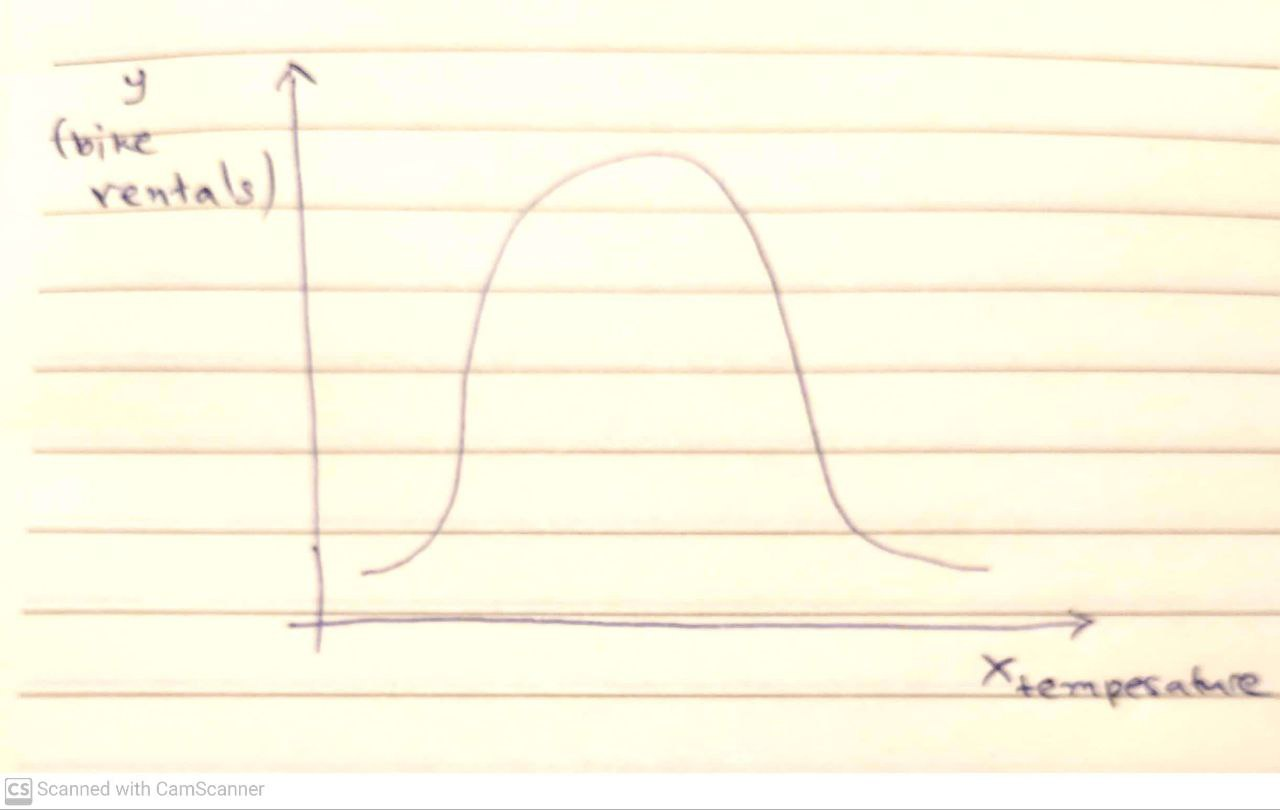
\includegraphics[width=0.7\textwidth]{./figures/gam_temperature.jpg}
  \end{figure}

\end{frame}


\begin{frame}
  \frametitle{GAMs - Interpretability}

  GAMs are explainable-by-design, why?

  \noindent\makebox[\linewidth]{\rule{\paperwidth}{0.4pt}}

  \begin{figure}[ht]
    \centering
    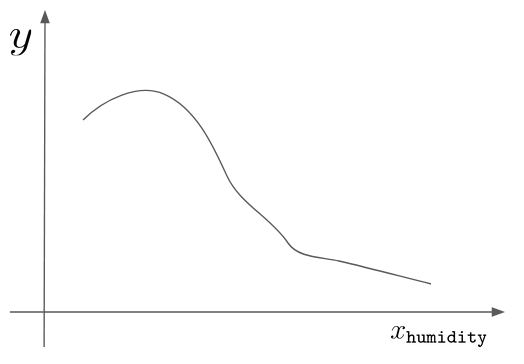
\includegraphics[width=0.7\textwidth]{./figures/gam_humidity.jpg}
  \end{figure}

\end{frame}

\begin{frame}
  \frametitle{GAMs - Interpretability}

  GAMs are explainable-by-design, why?

  \noindent\makebox[\linewidth]{\rule{\paperwidth}{0.4pt}}

  \begin{figure}[ht]
    \centering
    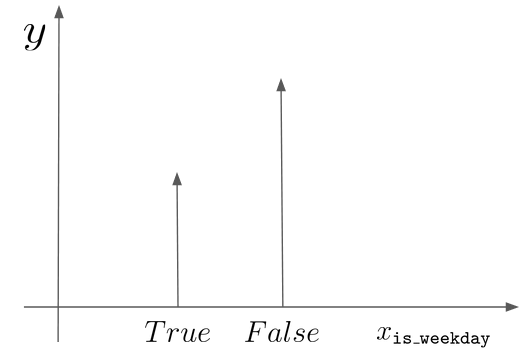
\includegraphics[width=0.7\textwidth]{./figures/gam_is_weekday.jpg}
  \end{figure}

\end{frame}

\begin{frame}
  \frametitle{GAMs - Interpretability}

  GAMs are explainable-by-design, why?

  \noindent\makebox[\linewidth]{\rule{\paperwidth}{0.4pt}}

  \begin{figure}[ht]
    \centering
    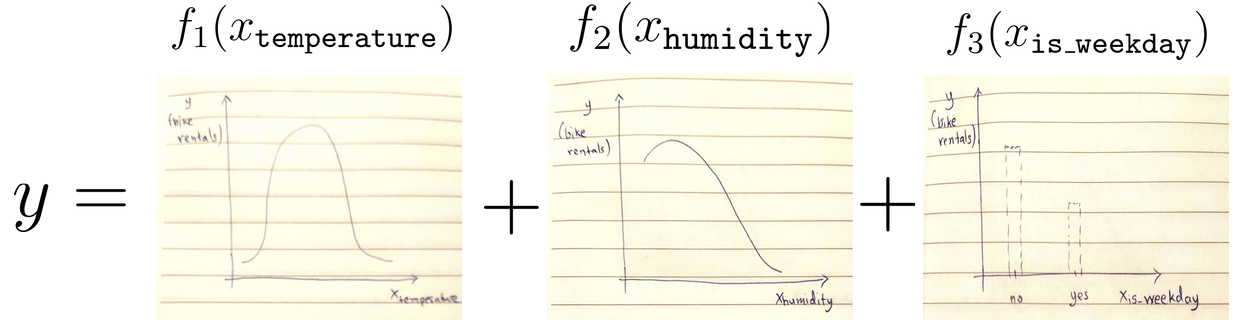
\includegraphics[width=0.7\textwidth]{./figures/additive_model.png}
  \end{figure}

\end{frame}


\begin{frame}
  \frametitle{GAMs - Limitations}

  What if:
  \begin{itemize}
  \item<1-> temperature has different effect on week-days vs weekends
  \item<2-> Cause: go to work vs go sightseeing
  \item<3-> Solution 1: \(f(x_{\mathtt{temperature}}, x_{\mathtt{is\_weekday}})\)
  \item<4-> Solution 2: \(f(x_{\mathtt{temperature}} | weekday )\) vs \(f(x_{\mathtt{temperature}} | weekend )\)
  \end{itemize}

  \noindent\makebox[\linewidth]{\rule{\paperwidth}{0.4pt}}
  \begin{itemize}
  \item<5-> Solution 1: \(GA^2M\)
  \item<6-> Solution 2: \(RAM\)
  \end{itemize}

\end{frame}


\begin{frame}
  \frametitle{GAMs - Limitations}

  What if:
  \begin{itemize}
  \item<1-> Have you ever rided a bike with cold and humidity?
  \item<2-> If it is weekend, cool! Netflix is here!
  \item<3-> But what to do if the only option to go to work?
  \end{itemize}

  \noindent\makebox[\linewidth]{\rule{\paperwidth}{0.4pt}}

  Solutions:

  \begin{itemize}
  \item<4-> \(f(x_{\mathtt{temperature}}, x_{\mathtt{humidity}} | x_{\mathtt{is\_weekday}})\) \textcolor{red}{\(RA^2M\)}
    \item<5-> \(f(x_{\mathtt{temperature}}| x_{\mathtt{humidity}} = \{high, low\}, x_{\mathtt{is\_weekday}})\) \textcolor{red}{RAM with two conditions}
  \end{itemize}

\end{frame}


\begin{frame}
  \frametitle{RAM on toy example}

  \[f(\xb) = 8x_2\when{x_1 > 0}\when{x_3=0}\]

  \[ x_1, x_2 \sim \mathcal{U}(-1,1), x_3 \sim Bernoulli(0,1)\]

  \noindent\makebox[\linewidth]{\rule{\paperwidth}{0.4pt}}

  \begin{figure}[htbp]
    \centering
    \begin{subfigure}{0.32\textwidth}
        \centering
        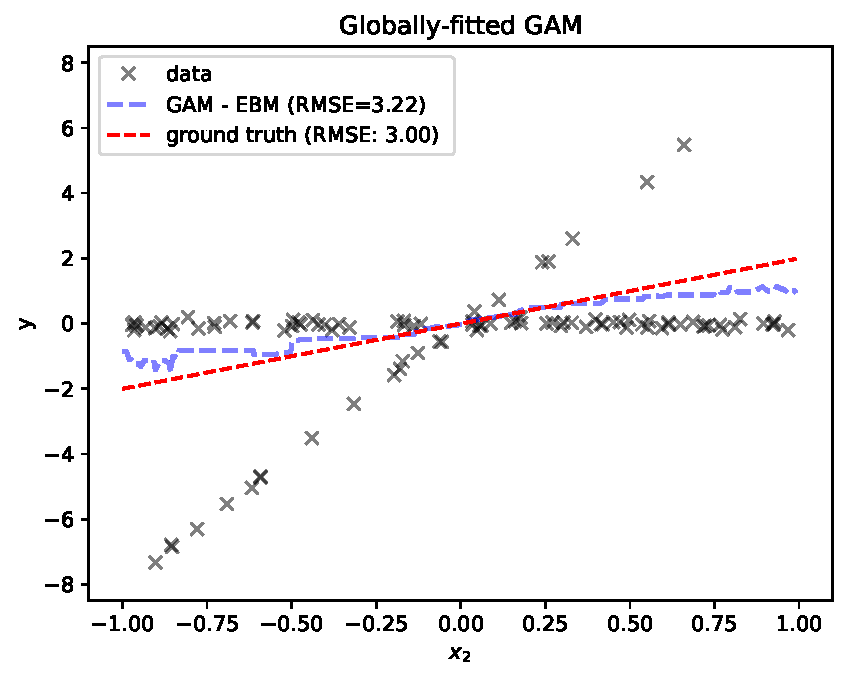
\includegraphics[width=\textwidth]{figures/global_GAM}
        \caption{\(f_2(x_2)\)}
        \label{subfig:global_gam}
    \end{subfigure}
    \begin{subfigure}{0.32\textwidth}
        \centering
        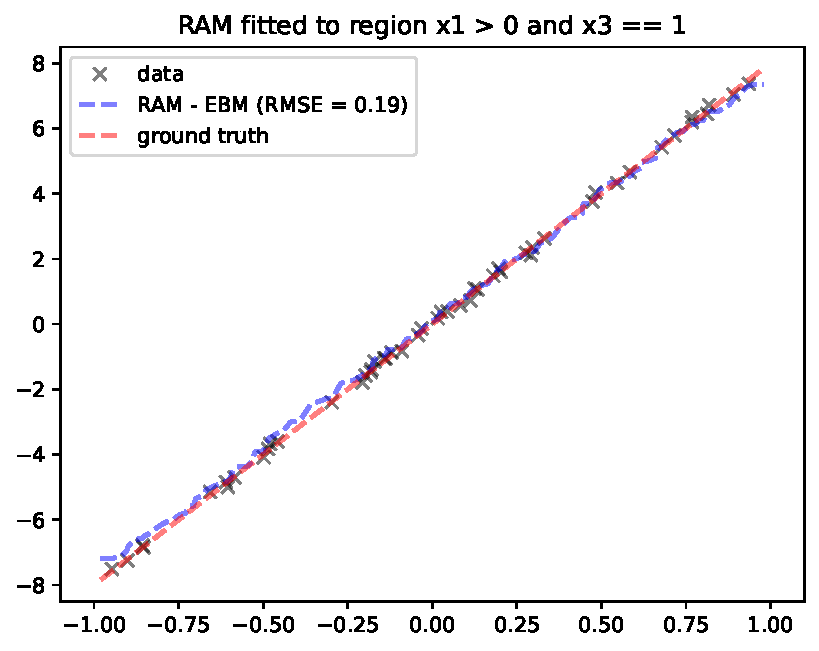
\includegraphics[width=\textwidth]{figures/regional_gam_subreg_1}
        \caption{\(f_2(x_2) \when{x_1 > 0 \text{ and } x_3 = 1}\)}
        \label{subfig:regional_gam_1}
    \end{subfigure}
    \begin{subfigure}{0.32\textwidth}
        \centering
        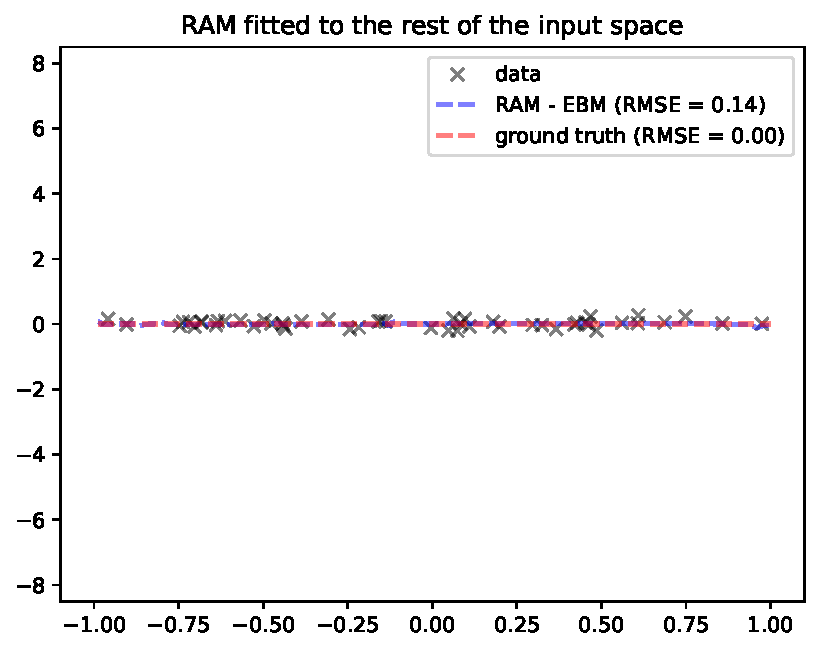
\includegraphics[width=\textwidth]{figures/regional_gam_subreg_2}
        \caption{\(f_2(x_2) \when{x_1 \leq 0 \text{ or } x_3 \neq 1}\)}
        \label{subfig:regional_gam_2}
    \end{subfigure}
    \caption{(Left) GAM, (Middle and Right) RAM}
    \label{fig:ram_example}
\end{figure}
\end{frame}


\begin{frame}
  \frametitle{How RAM works (1)}

  3-step approach:

  \begin{itemize}
  \item Fit a Black-box model to capture all complex structures
    \begin{itemize}
    \item it should be differentiable
    \item neural network
  \end{itemize}
\item Use a Regional Effect method to find important interactions
  \begin{itemize}
  \item \href{https://givasile.github.io/assets/pdf/gkolemis23_rhale.pdf}{RHALE - Gkolemis et. al}
  \item \href{https://arxiv.org/pdf/2306.00541.pdf}{Feature Interactions - Herbinger et. al}
  \end{itemize}

  \item Fit a univariate function on each detected subregion

  \end{itemize}

\end{frame}

\begin{frame}
  \frametitle{Step 1}
  \begin{itemize}
  \item Fit a Black-box model to capture all complex structures
    \begin{itemize}
    \item it should be differentiable
    \item A neural network is a good option
  \end{itemize}
\end{itemize}
\end{frame}

\begin{frame}
  \frametitle{Step 2}
  \begin{itemize}
  \item Use a Regional Effect method to find important interactions
    \begin{itemize}
    \item \href{https://givasile.github.io/assets/pdf/gkolemis23_rhale.pdf}{RHALE - Gkolemis et. al}
    \item \href{https://arxiv.org/pdf/2306.00541.pdf}{Feature Interactions - Herbinger et. al}
    \end{itemize}
  \end{itemize}
\end{frame}

\begin{frame}
  \frametitle{Step 3}
  \begin{itemize}
  \item Fit a univariate function on each detected subregion
    \begin{itemize}
    \item
    \end{itemize}
  \end{itemize}
\end{frame}

\begin{frame}
  \frametitle{Bike Sharing dataset}
  Predict bike-rentals (on daily basis) given some features of the day
  \noindent\makebox[\linewidth]{\rule{\paperwidth}{0.4pt}}
\begin{figure}[htbp]
    \centering
    \begin{subfigure}{0.32\textwidth}
        \centering
        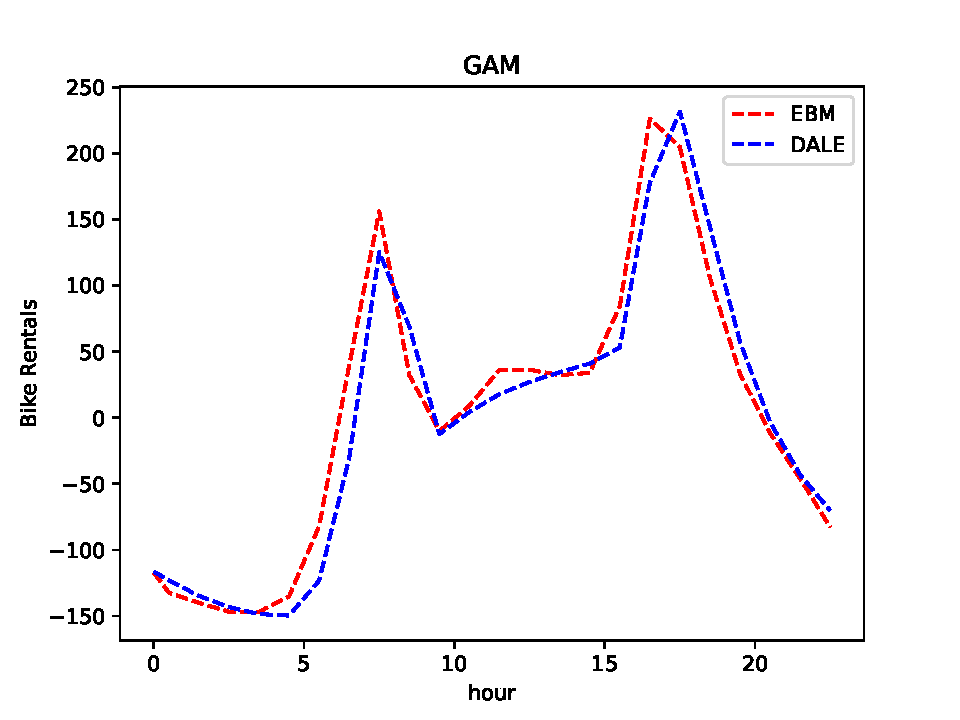
\includegraphics[width=\textwidth]{figures/bike_rentals_gam}
        \caption{\(f(X_{\mathtt{hour}})\)}
        \label{subfig:bike_rentals_gam}
    \end{subfigure}
    \begin{subfigure}{0.32\textwidth}
        \centering
        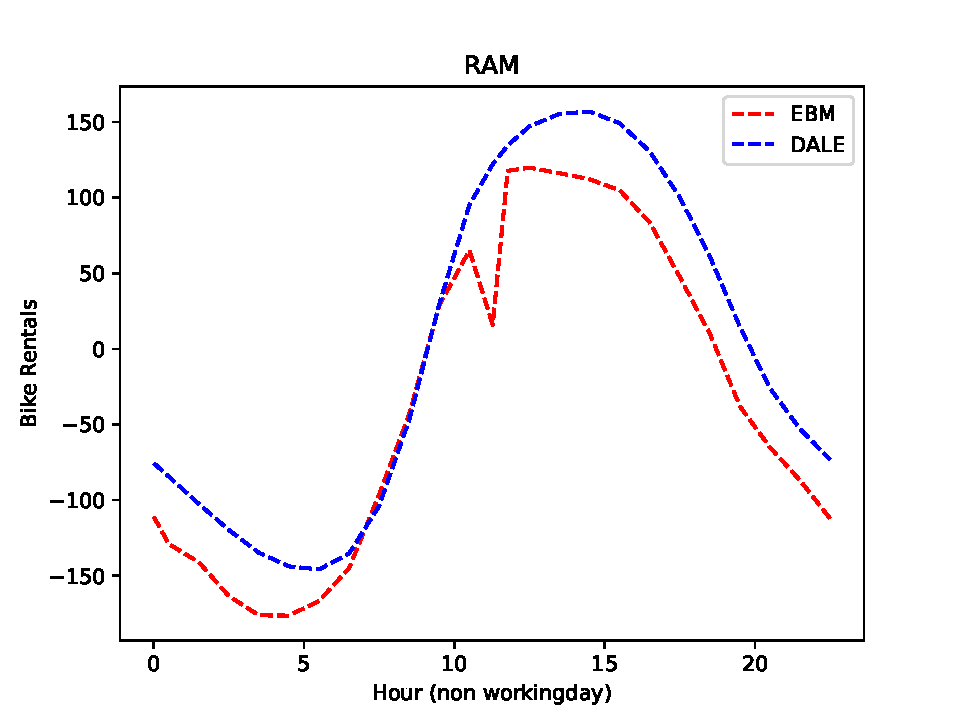
\includegraphics[width=\textwidth]{figures/bike_rentals_ram_1}
        \caption{\(f(X_{\mathtt{hour}}) \when{X_{\mathtt{workingday}} \neq 1}\)}
        \label{subfig:bike_rentals_regional_gam_1}
    \end{subfigure}
    \begin{subfigure}{0.32\textwidth}
        \centering
        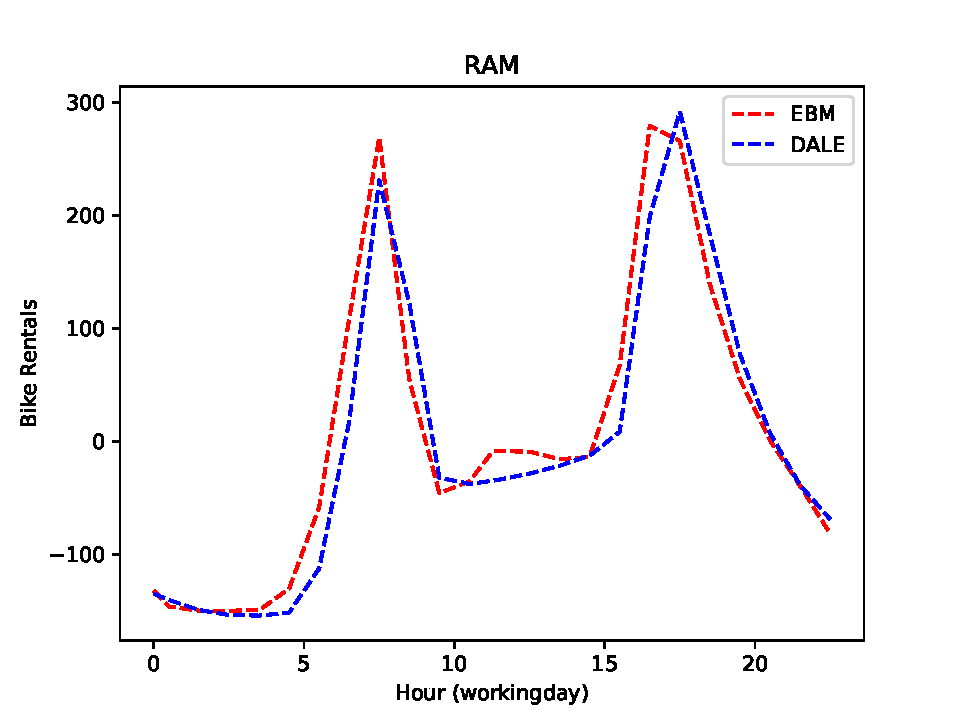
\includegraphics[width=\textwidth]{figures/bike_rentals_ram_2}
        \caption{\(f(X_{\mathtt{hour}}) \when{X_{\mathtt{workingday}} = 1}\)}
        \label{subfig:bike_rentals_regional_gam_2}
    \end{subfigure}
    \label{fig:bike_sharing}
\end{figure}

\end{frame}


\begin{frame}
  \frametitle{Experimental Results}

\begin{table}[htbp]
  \centering
  \label{tab:sample}
  \begin{tabular}{l|c|cccc}
      & \textbf{Black-box} & \multicolumn{4}{c}{\textbf{x-by-design}} \\
      \hline
      \hline
      & all orders & \multicolumn{2}{c}{1\textsuperscript{st} order} & \multicolumn{2}{c}{2\textsuperscript{nd} order} \\
      \hline
      \hline
      & \textbf{DNN} & \textbf{GAM} & \textbf{RAM} & \textbf{GA}$^2$\textbf{M} & \textbf{RA}$^2$\textbf{M} \\
      \hline
      Bike (MAE)  & 0.254 & 0.549 & 0.430 & 0.298 & 0.278 \\
      Bike (RMSE) & 0.389 & 0.734 & 0.563 & 0.438 & 0.412 \\
      \hline
      Housing (MAE)  & 0.373 & 0.600 & 0.553 & 0.554 & 0.533 \\
      Housing (RMSE) & 0.533 & 0.819 & 0.754 & 0.774 & 0.739 \\
  \end{tabular}
\end{table}

\end{frame}


\begin{frame}
  \frametitle{What next?}
  A lot has to be done!
  \begin{itemize}
  \item Results are only preliminary
    \begin{itemize}
      \item Experiment with more datasets
      \item Sometimes wide bins are needed
      \end{itemize}
    \item Can we learn uncertain RAMs?
      \begin{itemize}
      \item How do we model uncertainty?
      \end{itemize}
  \end{itemize}

  \noindent\makebox[\linewidth]{\rule{\paperwidth}{0.4pt}}

\end{frame}


\begin{frame}
  \frametitle{Thank you for the attention}
  \begin{itemize}
  \item For more discussion or future ideas on RAM, contact me:
    \begin{itemize}
    \item \href{vgkolemis@athenarc.gr}{vgkolemis@athenarc.gr}
      \item \href{gkolemis@hua.gr}{gkolemis@hua.gr}
    \end{itemize}
  \item Questions?
  \end{itemize}
\end{frame}



% \begin{frame}[allowframebreaks]
%   \frametitle{References}
%   \printbibliography
% \end{frame}


\end{document}